\chapter{IMGuiViewer}
Je grafický \textbf{viewer}, který zobrazuje simulované objekty ve 2D a dovoluje ovládání simulace pomocí uživatelského rozhraní. Jeho implementace je rozdělena do relativně velkého množství tříd a využívá externí knihovny, které si představíme jako první.

\section{Třída \texttt{OpenGLBackend} a GLFW\&GLEW}
Tento program používá k vykreslování grafiky OpenGL, tato třída má na starosti jeho správnou inicializaci. Používá k tomu knihovnu \textbf{GLFW} a \textbf{GLEW}.
GLFW\footnote{http://www.glfw.org/} poskytuje funkce k vytvoření okna do kterého může poté OpenGL kreslit.
GLEW\footnote{http://glew.sourceforge.net/} se stará o získání OpenGL funkcí, které se musí načíst za běhu aplikace z konkrétních grafických ovladačů na cílovém počítači.
Přesná implementace je dostupná ve zdrojových kódech programu. Ale jedná se ve větší míře o přepsání doporučené implementace na stránkách obou knihoven.

\subsection{Třída \texttt{Shader}}
Slouží pro jednoduší vytváření OpenGL shaderů, tedy malých programů určených pro grafickou kartu, které říkají jak má interpretovat a kreslit předaná data.
\subsection{Řešení OpenGL chyb} 
OpenGL samo nemá výjimky a chyby sděluje pomocí funkce \texttt{glGetError()}, která vrací typ chyby pokud nějaká nastala. Proto byla vytvořena funkce \texttt{ThrowOnError}, která zavolá \texttt{glGetError()} a při jakékoliv chybě vyvolá výjimku právě v podobě třídy \texttt{GLError} s informacemi o chybě.
\subsection{Třída \texttt{ImGuiBackend} a ImGui}
Se stará o integraci knihovny \textbf{ImGui}\footnote{https://github.com/ocornut/imgui}, která poskytuje nástroje k vytvoření uživatelského rozhraní.
Její implementace byla také vytvořena na základě příkladů uvedených na stránkách knihovny a dokumentace v souborech \texttt{imgui.h} a \texttt{imgui.cpp}.
Pojďme si v rychlosti představit nějaké funkce knihovny, abychom pak lépe pochopili její použití při tvorbě uživatelského rozhraní.

\textbf{ImGui} je psáno v C++ ale z vnějšího pohledu vypadá spíše jako C, nejsou zde žádné složité třídy a většina prvků je z vnějšku bezstavová až na pár výjimek a např. funkce na výpis textu používá syntaxi podobnou \texttt{printf()}.

Zaprvé je ještě nutné zmínit jak OpenGL funguje. Ve zjednodušeném pohledu vykresluje do svého framebufferu( 2D plátno/textura) všechny objekty, které pak zobrazí na obrazovku. Toto plátno si můžeme a musíme mazat sami kdykoliv potřebujeme, pokud bychom ho nemazali, tak na něm zůstanou objekty z \uv{minulého} kreslení.
\footnote{Například by zde zůstali minulé pozice všech objektů, což je velmi rychlý způsob jak implementovat \ref{sec:unitTrail}, ale časem by to bylo velmi nepřehledné. Na druhou stranu to OpenGL nemůže dělat za nás, protože neví které volání kreslících funkcí ještě patří do \uv{tohoto} času a co už bylo \uv{minule}.} Takže si nejdříve vždy vyčistíme plátno a pak do něj vše nakreslíme a tento postup opakujeme ve smyčce.

\textbf{ImGui} má podobný systém, což je ukázáno na příkladu \ref{lst:imgui1}, na kterém si nyní vysvětlíme jak funguje.
\includecode[imgui1]{Source/imgui1.cpp}
{Příklad použití knihovny ImGui }
Vnější smyčku nám v programu už obstarává samotná simulace, takže o ní se starat nemusíme. Dále je zde dvojice funkcí \texttt{NewFrame()} a \texttt{Render()}, kde po zavolání \texttt{NewFrame()} si \textbf{ImGui} zaznamenává všechny další volání všech svých funkcí. \texttt{Render()} pak předá zaznamenaná data OpenGL, které je vykreslí na obrazovku. 

Tento konkrétní příklad vykresluje okno s jedním tlačítkem, které po zmáčknutí zobrazí text. Všimněme si, že zde není žádný objekt - tlačítko, okno, ani text. Vše je pouze volaní funkcí, což je klíčové pro pochopení fungování knihovny. Také je to důvod pro \texttt{if}, protože \uv{Foo} text se zobrazí jen a \textbf{pouze při konkrétním průchodu smyčkou}, ve kterém došlo k zmáčknutí tlačítka (reprezentováno návratovou hodnotou). Ve výsledku text na obrazovce jen problikne, samozřejmě v tomto případě asi chceme spíše přepínací tlačítko, k čemuž slouží jiná funkce. Také se vše zobrazí jen a pouze pokud je okno otevřené, což je jedna z výjimek, kde si \textbf{ImGui} uchovává stav. Nic nám ovšem nebrání tuto funkci občas nezavolat, což bude znamenat, že se nám okno občas nevykreslí vůbec. Tento přístup dovoluje rychlý vývoj a velkou dynamičnost uživatelského rozhraní. Ze zdrojového kódu je tedy hned patrné co, kdy a za jakých podmínek se bude kreslit.

Většina funkcí využívající \textbf{ImGui} by teď už měla být alespoň koncepčně jasná, pokud ne, tak knihovna je dobře okomentovaná a když tak není problém si najít volné místo v našem kódu, a některé funkce si jen tak vyzkoušet, což je díky bezstavové implementaci velmi snadné. Popřípadě na stránkách knihovny je předpřipravený projekt, ve kterém se dá kód rychle otestovat a také je tam interaktivní demo se zdrojovými kódy představující jednotlivé funkce.
\section{Kreslení simulace}
Nyní představíme pár tříd, které se starají o vykreslení samotných simulovaných dat
\subsection{třída \texttt{OMSAR}}
\texttt{OMSAR}(z Offset-Move-Scale-Aspect-Ratio) slouží k transformaci mezi souřadnou soustavou simulovaných dat a normalizovanými souřadnicemi, které využívá OpenGL. Jedná se o třídu ze které mají ostatní třídy zdědit sadu funkcí, která právě popsanou transformaci zajišťuje. Pomocí této třídy je také zajištěno posouvání obrazovky a přibližování/oddalování, což se děje pomocí dvou proměnných \texttt{Vec2 offset}(posouvání) a \texttt{scale}(přibližování). Tyto dvě proměnné využívají ostatní třídy, aby si správně posunuly vykreslované prvky na obrazovku.
\subsection{třídy \texttt{CircleBuffer} a \texttt{SimDataDrawer}} 
První jmenovaná třída umí vykreslit kruh o zadaném poloměru do středu obrazovky. K tomu využívá prvky OpenGL - konkrétně \textbf{buffery}. Pro posouvání se musí použít správný \textbf{shader}.
 
Druhá jmenovaná třída vykresluje data, kde jednomu objektu odpovídá právě jeden \texttt{CircleBuffer} - kruh. Data vykresluje pomocí funkce \texttt{Draw()}, která zajišťuje správný \textbf{shader} a využívá právě \texttt{OMSAR} k určení polohy jednotlivých kruhů.
\subsection{třída \texttt{UnitTrail}}
\label{sec:unitTrail}
Při simulaci Sluneční soustavy by se nám hodilo nejen vidět aktuální polohu všech objektů, ale i jejich minulé polohy. Tato třída vykresluje lomenou čáru, která pak slouží jako \uv{stopa} za simulovaným objektem. Ideálně bychom chtěli mít pouze funkci, která přidá další bod lomené čáry a to aktuální polohu. O to jak bude stopa uložena a kreslena se z vnějšku starat nechceme. Samozřejmě bude omezená maximální délku, ale to si má také ohlídat sama. Ještě pro úplnost existuje funkce \texttt{Clear}, která uloženou čáru smaže.

\paragraph{Algoritmus}Využijeme toho, že OpenGL přímo podporuje kreslení lomených čar, stačí zadat množinu bodů a ono samo mezi nimi vykreslí lomenou čáru. Navíc použijeme indexované vykreslování, tedy, že řekneme OpenGL v jakém pořadí má body vykreslit, což ve výsledku zajistí, že celá množina bodů nemusí ležet ve správném pořadí a při přidávání bodů ji nebude nutné celou posouvat.


Mějme dvě pole - bodů velikosti \textbf{n} a indexů o délce \textbf{2n}.
Dále máme objekt, který postupně projde body \textbf{A-B-C-D-E-F}. Tak pokud za ním chceme vykreslit stopu(lomenou čáru) o maximálně \textbf{n} bodech. Pak vytvoříme funkci \texttt{Push(Bod b)}, která umístí předaný bod do pole bodů. Pokud už je plné tak začne přepisovat body od začátku. Pole indexů vyplníme čísly od \textbf{1} do \textbf{n} dvakrát. Obrázek \ref{fig:lineTrail} popisuje jak bude algoritmus pro náš objekt fungovat při projití všech bodů, kde v každém bodě zavoláme \texttt{Push(bod)} a délka stopy je \textbf{n=3}.

\begin{figure}
	\caption{Kreslení stopy za objektem procházejícím body A-B-C-D-E-F}
	\label{fig:lineTrail} 
	\centering
	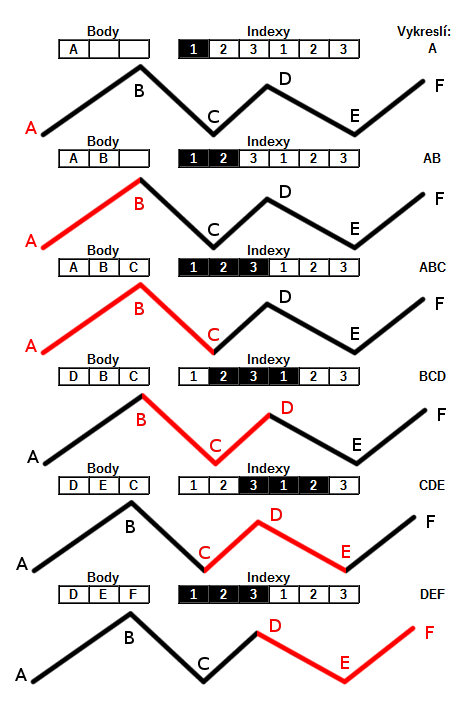
\includegraphics[width=0.5\linewidth]{Figs/LineTrail}\\
	\textit{Obrázek zobrazuje postupné(shora dolů) přidání 6 bodů do stopy o maximální délce 3. Červeně je vykreslena aktuální stopa. Pokud jsou černě vyplněné např. indexy(indexováno od jedničky) 2,3,1. Tak to znamená, že se vykreslí přímka v pořadí: \lstinline|body[2],body[3],body[1]|(což je napsáno vpravo).}
\end{figure}
\FloatBarrier
Z obrázku si můžeme všimnout, že si musíme držet pouze ukazatel na prvek v poli bodů, kam budeme vkládat, a ukazatel na index v poli indexů od kterého máme kreslit. Oba ukazatele pak budeme vždy pouze cyklicky posouvat a odpadne tím nutnost přesouvat celé pole při přidání jednoho bodu.
\\

\textbf{Poznámka:}\textit{Teoreticky žádné indexy nepotřebujeme a mohli bychom kreslit vždy pouze úsečky. Ale zavolání jednoho vykreslení je v OpenGL relativně drahé, proto je lepší kreslit co nejvíce dat jedním příkazem. Proto také máme jeden kontinuální buffer pro všechny body. Tento algoritmus tedy považuji za kompromis mezi rychlostí a čitelností kódu. Teoreticky také stačí index buffer o velikosti \textbf{n} a pak čáru kreslit na dvakrát, protože je v bufferu buď uložená kontinuálně a nebo rozložená do dvou částí. Což by byla rozumná paměťová optimalizace, ale indexy zas tolik místa nezabírají a navíc existuje pouze jeden globální indexový buffer pro všechny instance třídy \texttt{UnitTrail} neboť je jen pro čtení.}

\subsection{Třída \texttt{LineTrailsDrawer}}
Tato třída vytvoří pro každý simulovaný objekt jednu \texttt{UnitTrail}, do kterých pak periodicky ukládá jejich pozice a také všechny stopy vykresluje, k čemuž používá správný shader a informace z \texttt{OMSAR}. Nabízí také pár kontrolních funkcí jako selektivní mazání/vypínání/zapínání stop pro jednotlivé objekty.

\section{Kreslení uživatelského rozhraní}
Celé uživatelské rozhraní využívá plně knihovnu \textbf{ImGui} a je rozděleno do několika následujících souborů.
\begin{description}
	\item[MouseControls] Skupina funkcí, která implementuje ovládání pomocí myši. Tedy posouvání obrazovky a přibližování/oddalování.
	\item[SimProperties] Skupina funkcí, které vykreslují okno s informacemi o simulaci a také dovolují simulaci ovládat.
	\item[Visuals] Skupina funkcí, která vykresluje okno s ovládáním grafických prvků, tedy momentálně pouze kreslení stop za objekty. Dovoluje stopy selektivně vypínat/zapínat/mazat pro všechy objekty.
	\item[UnitsProperties] třída, která vykresluje okno, které zobrazuje fyzikální informace o vybraném objektu.
\end{description}
Koncepčně na těchto třídách/funkcích není nic moc zajímavého. Ze zdrojových kódů a názvů funkcí v nich je celkem jasné co dělají.
